\documentclass[pdf]{beamer}
\usepackage{caption}

\title{Modeling of spin-orbital dynamics in a FS lattice with E+B in the same element}
\author{Alexander Aksentev}

\begin{document}
	\begin{frame}
		\titlepage
	\end{frame}	

	\begin{frame}
		\frametitle{Tasks from supervisor}
		\begin{itemize}
			\item Study effects of E+B tilts (preserves Lorentz force) in FS lattice on $S_x, S_y, S_z$;
			\item Same for quadrupole shifts (doesn't preserve LF in the quadrupole);
			\item Study decoherence as a function of the inital beam distribution ($x, y, \delta W$);
			\item Study optimal sextupole placement for the suppression of decoherence and chromaticity;
			\item Modeling of field calibration by effective gamma in the horizontal plane (CW/CCW procedure);
		\end{itemize}
	\end{frame}

	\begin{frame}
		\frametitle{Conventional ODE integrator}
		\framesubtitle{Python prototype}
		\begin{itemize}
%			\item Wrote that because couldn't get COSY INFINITY to produce results that I could interpret;
			\item Classes defining most commonly utilized accelerator elements (dipoles, quadrupoles, E+B, etc);
			\item Vectorized RHS computation;
			\item Two versions of element positioning imperfections (tilting):
			\begin{itemize}
				\item via computing the tilt matrix, and applying it to the computed field at run time (more general but time-consuming, doesn't preserve guiding field strength by default);
				\item customized tilting for dipole, E+B (less time-consuming, preserves the Lorentz force acting on the particle), and shift for quadrupole;
			\end{itemize}
		\item Reason: needed a tool whose output could be exactly interpreted (source code could be understood by \emph{me})
		\end{itemize}
	\end{frame}

%	\begin{frame}
%		\frametitle{Example plots}
%		\begin{columns}
%			\column{.5\textwidth}
%			\begin{itemize}
%				\item $S_x \sim s$ in FS lattice w/o tilt
%				\item $S_x \sim s$ in FS structure w/ all elements tilted about $\hat s$
%				\item $S_y \sim s$ in FS structure w/ elements randomly tilted Norm(0, $10^{-4}$ rad)
%			\end{itemize}
%			\begin{minipage}{.3\textheight}
%				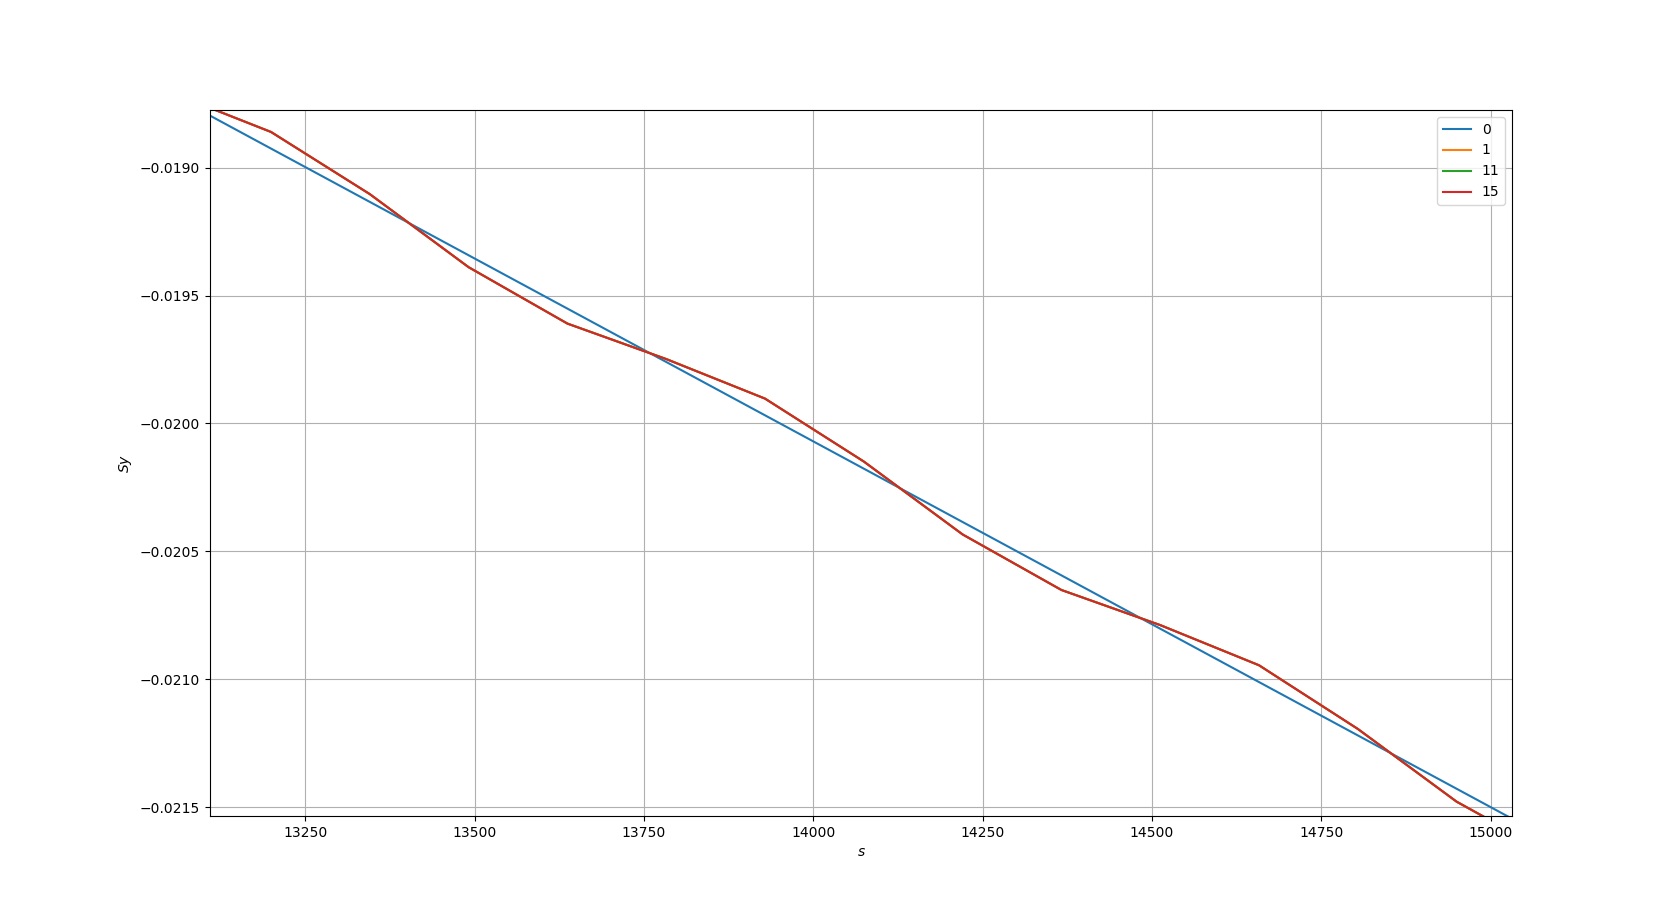
\includegraphics[scale=.15]{Sy_300_sigma_tilts_0057_deg_piece}
%			\end{minipage}
%			\column{.5\textwidth}
%			\begin{minipage}{.3\textheight}
%				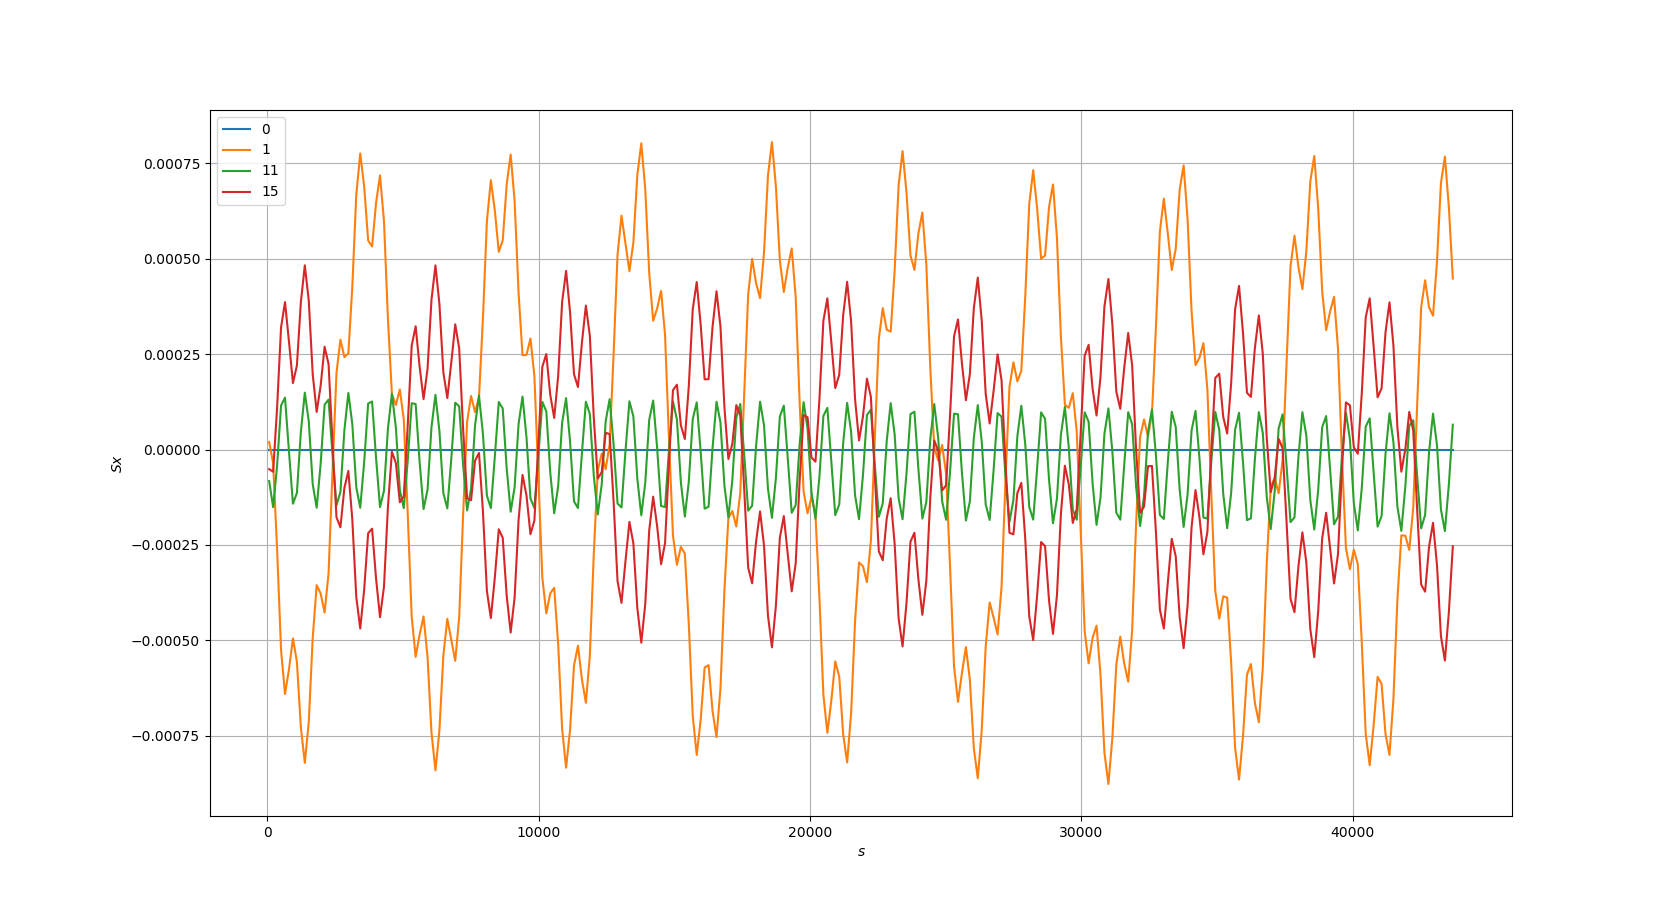
\includegraphics[scale=.15]{Sx_300_no_tilt}
%			\end{minipage}
%			\begin{minipage}{.3\textheight}
%				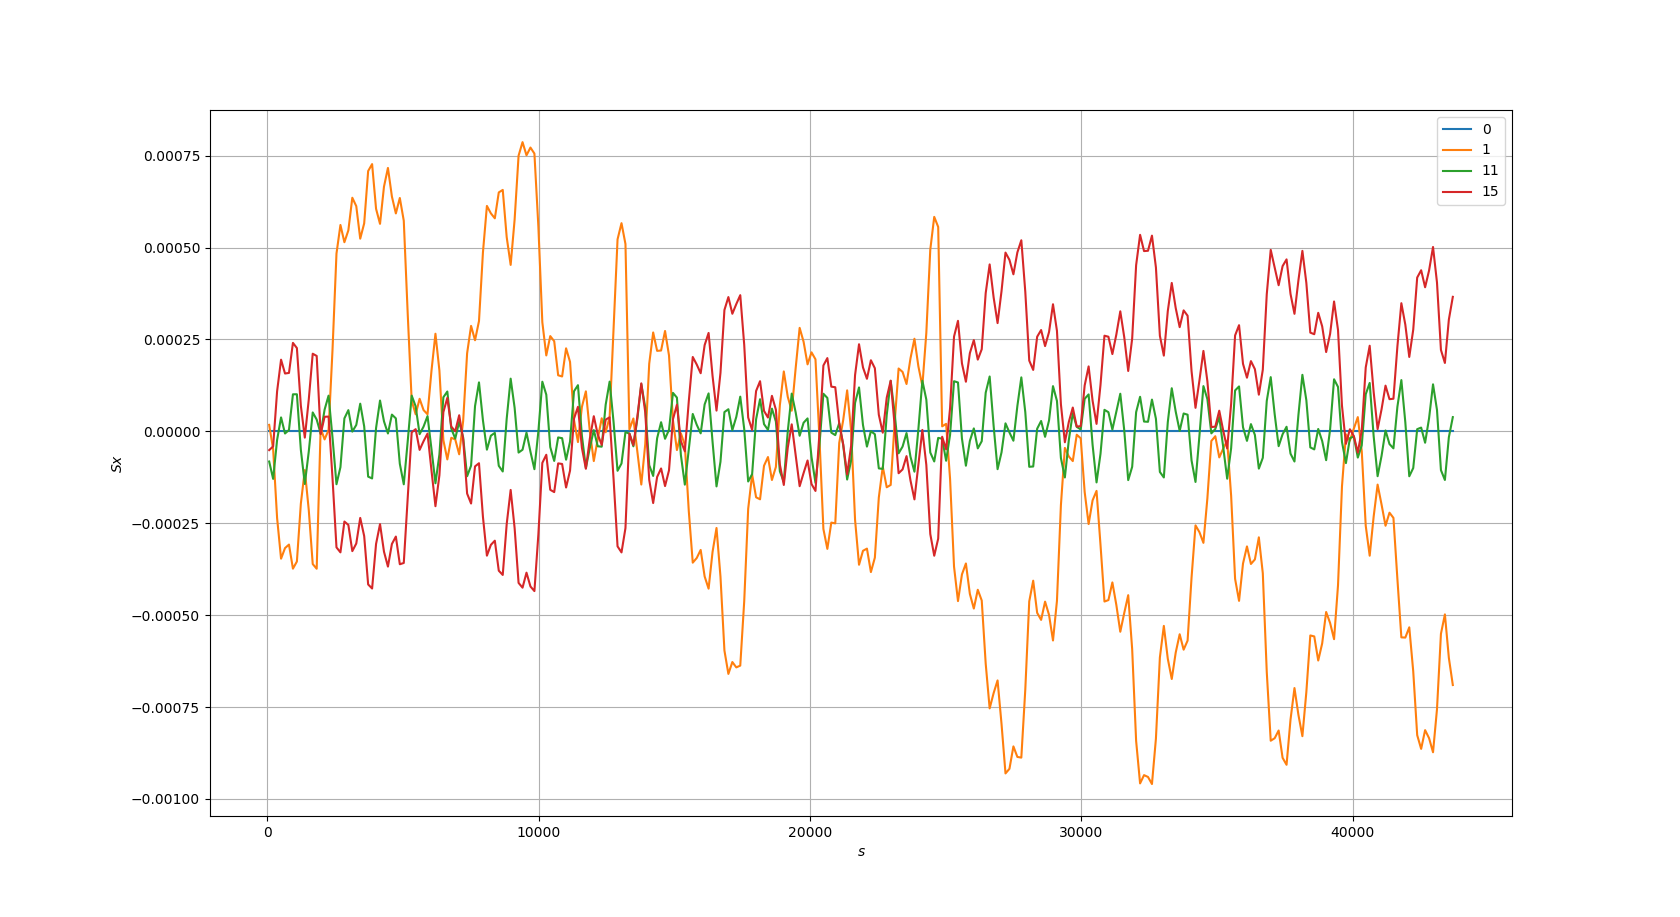
\includegraphics[scale=.15]{Sx_300_all_tilts_3_6}
%			\end{minipage}
%		\end{columns}
%	\end{frame}

	\begin{frame}
		\frametitle{Decoherence test}
		\begin{itemize}
			\item 1000 initial conditions from $\Delta K \sim N(0, 10^{-4})$;
			\item $\vec{S}(0) = (0,0,1)$;
			\item Tracking for the first 100 turns;
			\item Statistics: $\Omega_x = S_y(100) / \Delta t(100), ~ \Omega_y = S_x(100) / \Delta t(100)$.
		\end{itemize}
	\end{frame}
	\begin{frame}
		\centering
		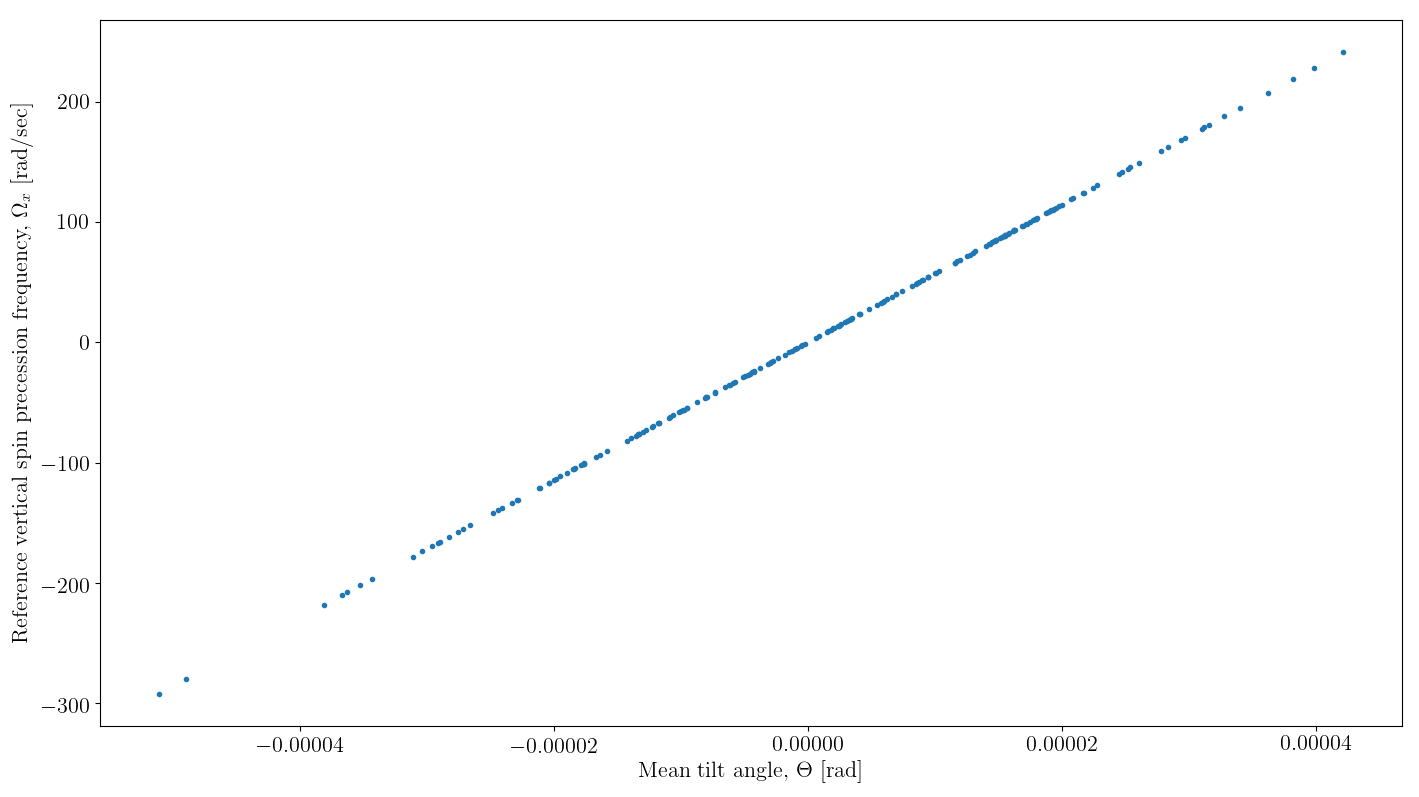
\includegraphics[scale=.3]{Wx_dK_reference_vs_tilt_mean_cut}
		\captionof{figure}{Reference particle spin precession frequency (vertical plane) vs mean tilt angle}
	\end{frame}
	\begin{frame}
		\centering
		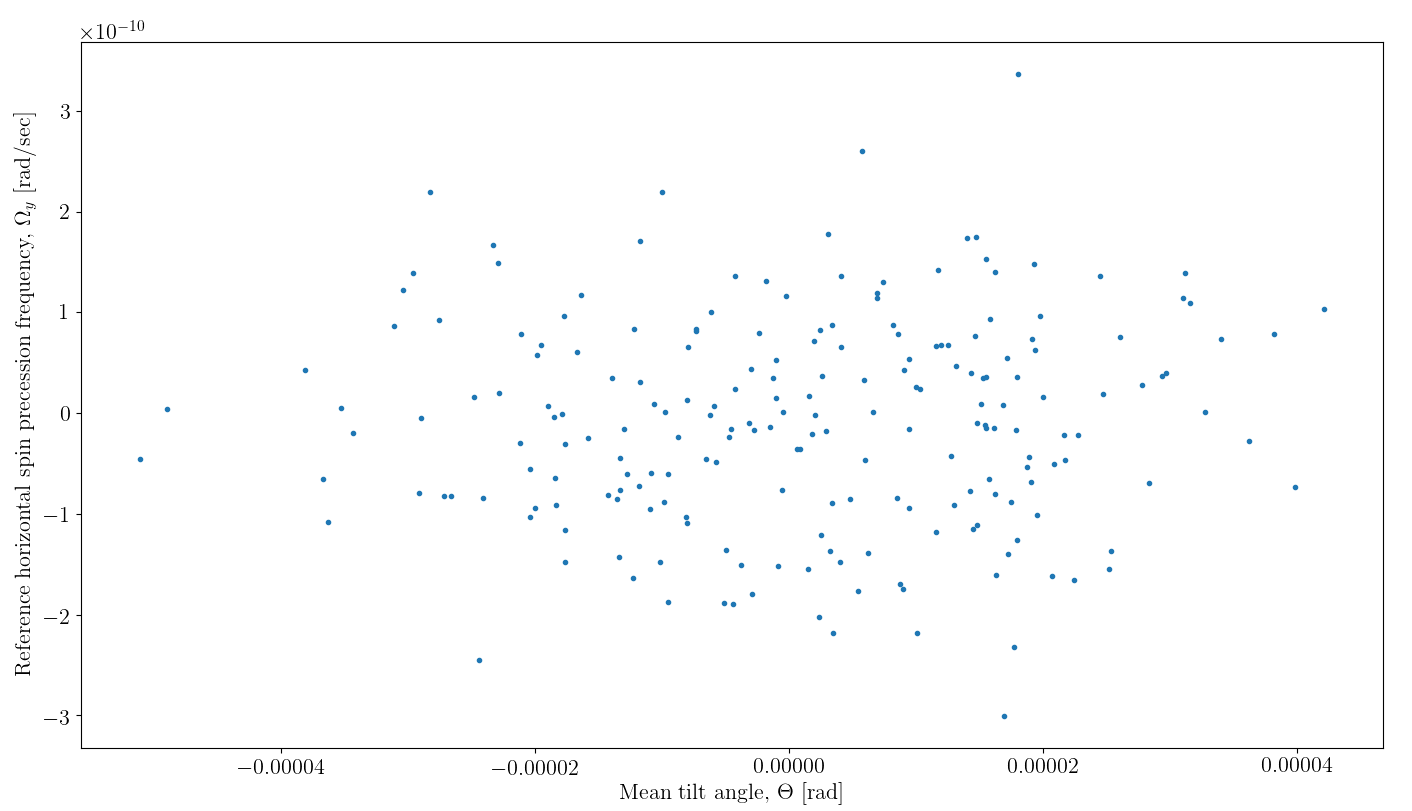
\includegraphics[scale=.3]{Wy_dK_reference_vs_tilt_mean_cut}
		\captionof{figure}{Reference particle spin precession frequency (horizontal plane) vs mean tilt angle}
	\end{frame}
	\begin{frame}
		\centering
		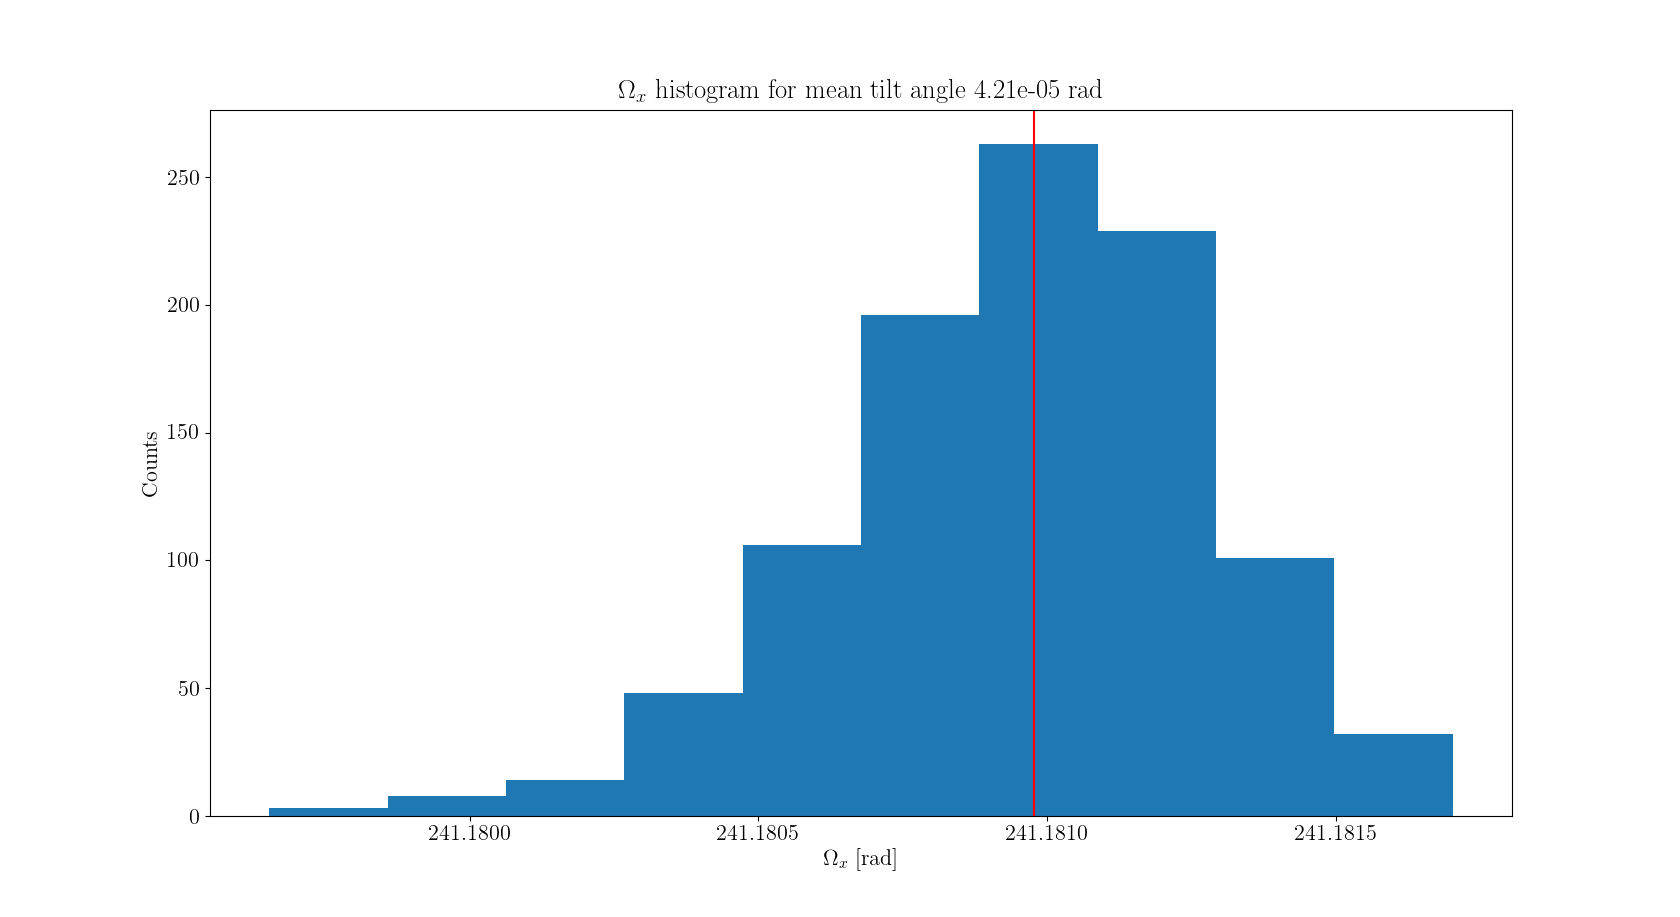
\includegraphics[scale=.3]{Wx_dK_hist_most_positive_mean_tilt}
		\captionof{figure}{Vertical spin precession frequencies at the most positive mean tilt; red: reference particle}
	\end{frame}
	\begin{frame}
		\centering
		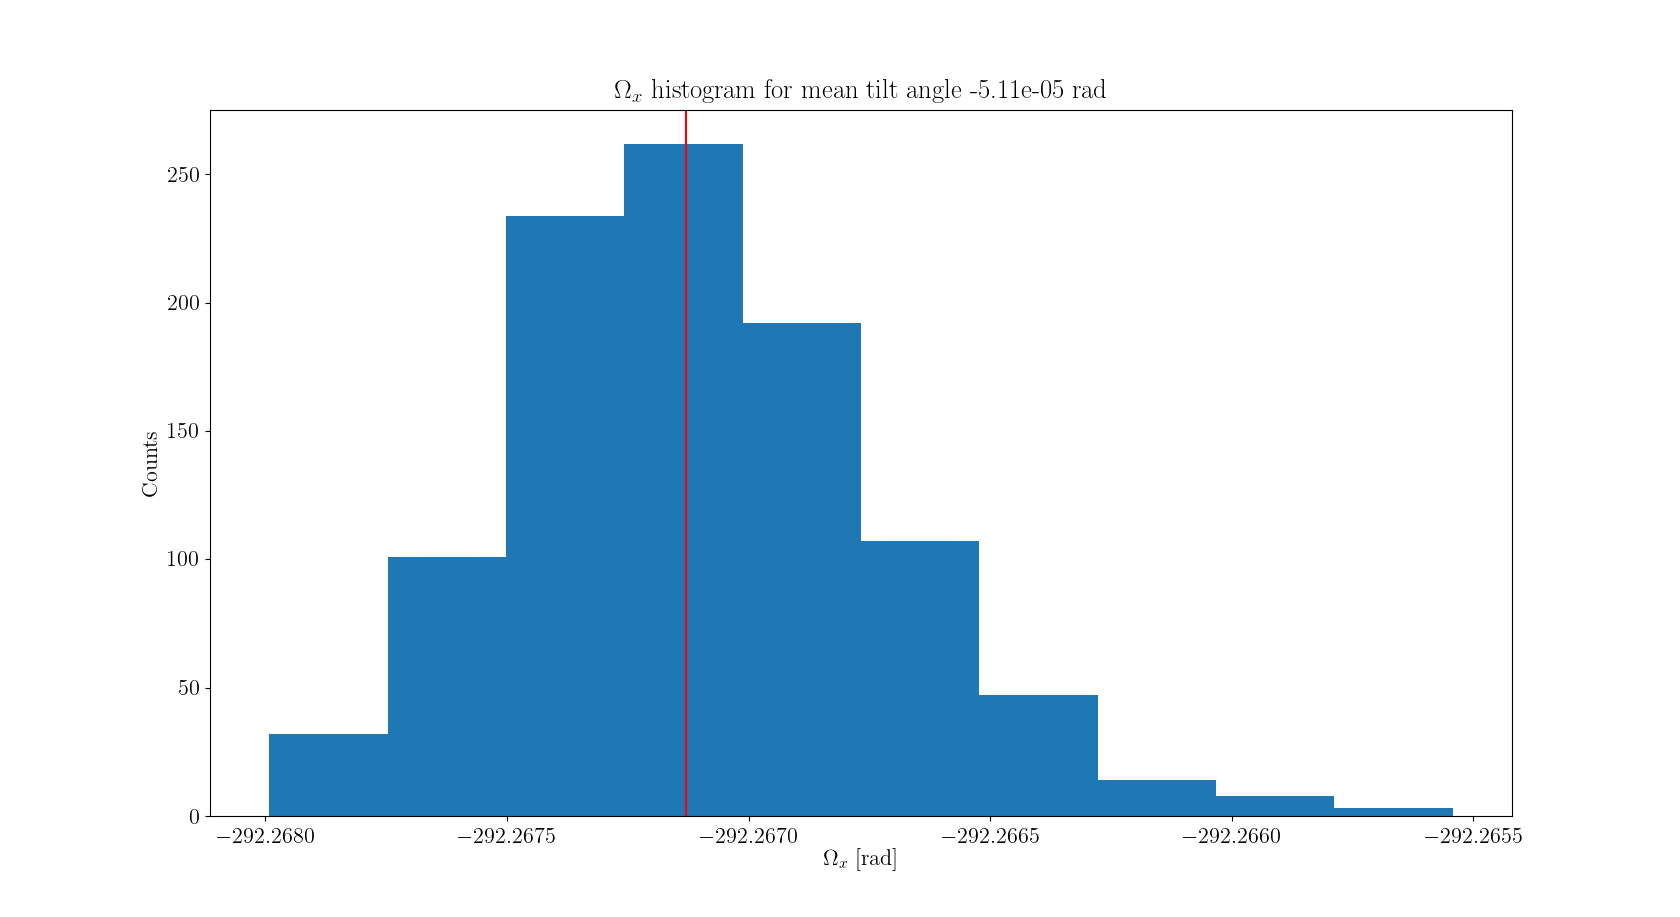
\includegraphics[scale=.3]{Wx_dK_hist_most_negative_mean_tilt}
		\captionof{figure}{Vertical spin precession frequencies at the most negative mean tilt; red: reference particle}
	\end{frame}
	\begin{frame}
		\centering
		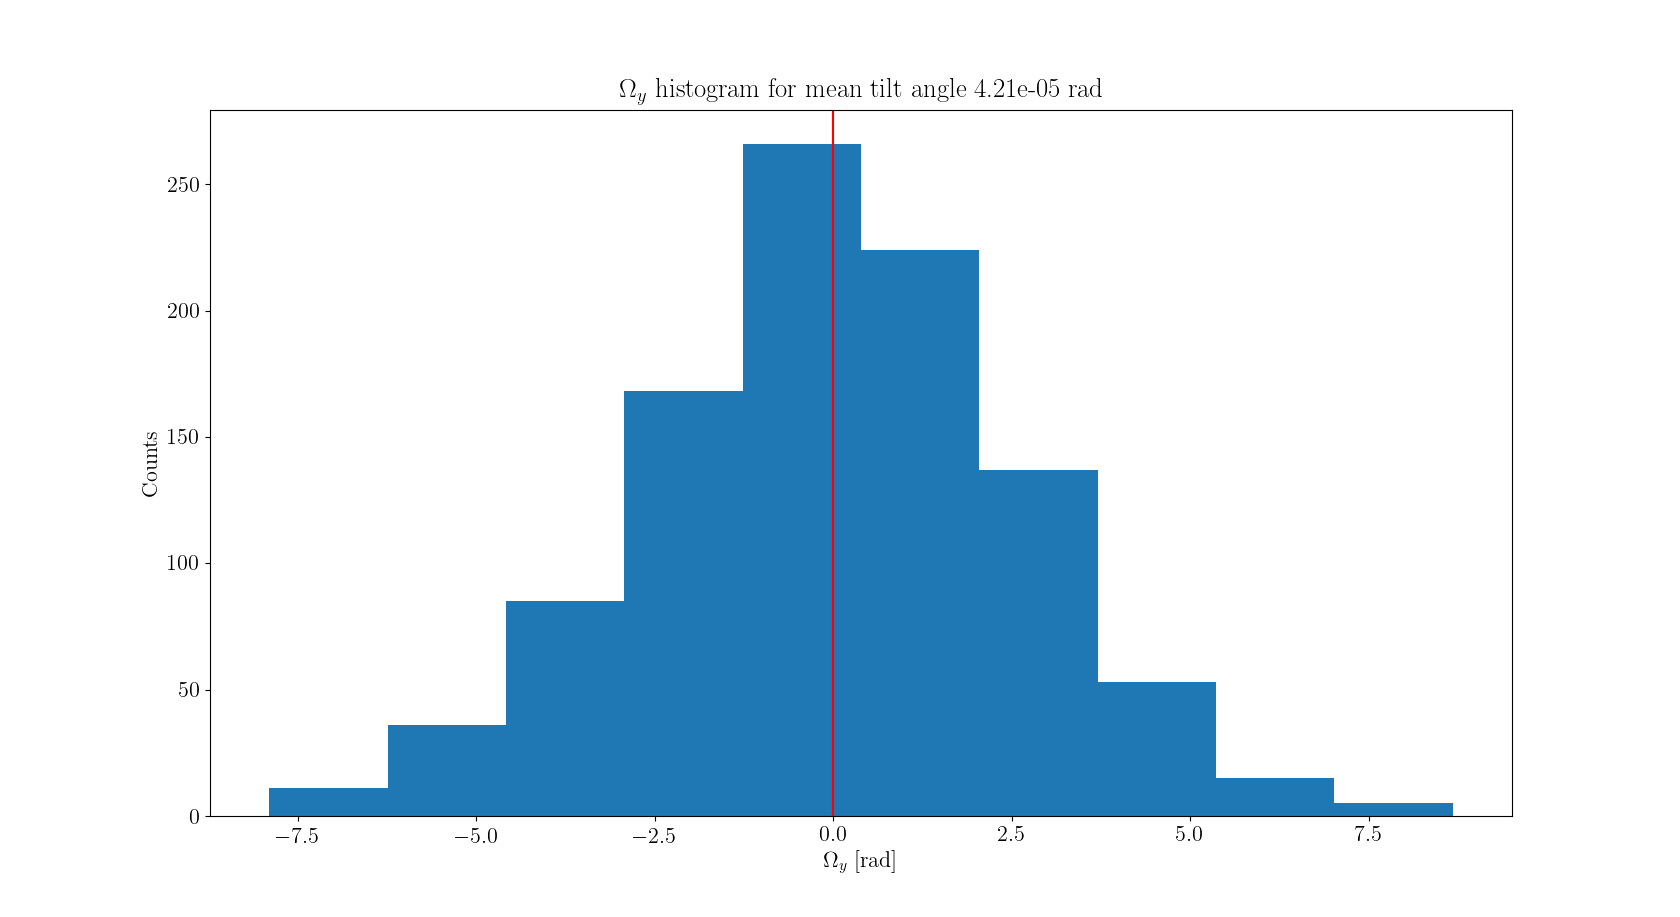
\includegraphics[scale=.3]{Wy_dK_hist_most_positive_mean_tilt}
		\captionof{figure}{Horizontal spin precession frequencies at the most positive mean tilt; red: reference particle}
	\end{frame}
	\begin{frame}
		\frametitle{Conventional ODE integrator}
		\framesubtitle{C++ extension}
		\begin{itemize}
			\item Because python isn't fast enough, rewrote parts of the integrator in c++;
			\item Still problems with speed (and precision) --- working on that now;
			\item However, even if those problems are resolved, step-by-step integration is not a viable option for the type of analysis required:
		\end{itemize}
	\end{frame}
	\begin{frame}{What is required?}
			\begin{itemize}
				\item $\omega_i = \omega_0 + G_6\cdot\Delta\gamma_i^2$, where $\Delta\gamma_i^2$ is the average gamma in phase space, due to synchrotron oscillations.
				\item $Q_s = \frac{\omega_s}{\omega_{rev}} \ll 1$ (like 1/35) $=>$ require thousands of turns.
			\end{itemize}
		\centering
		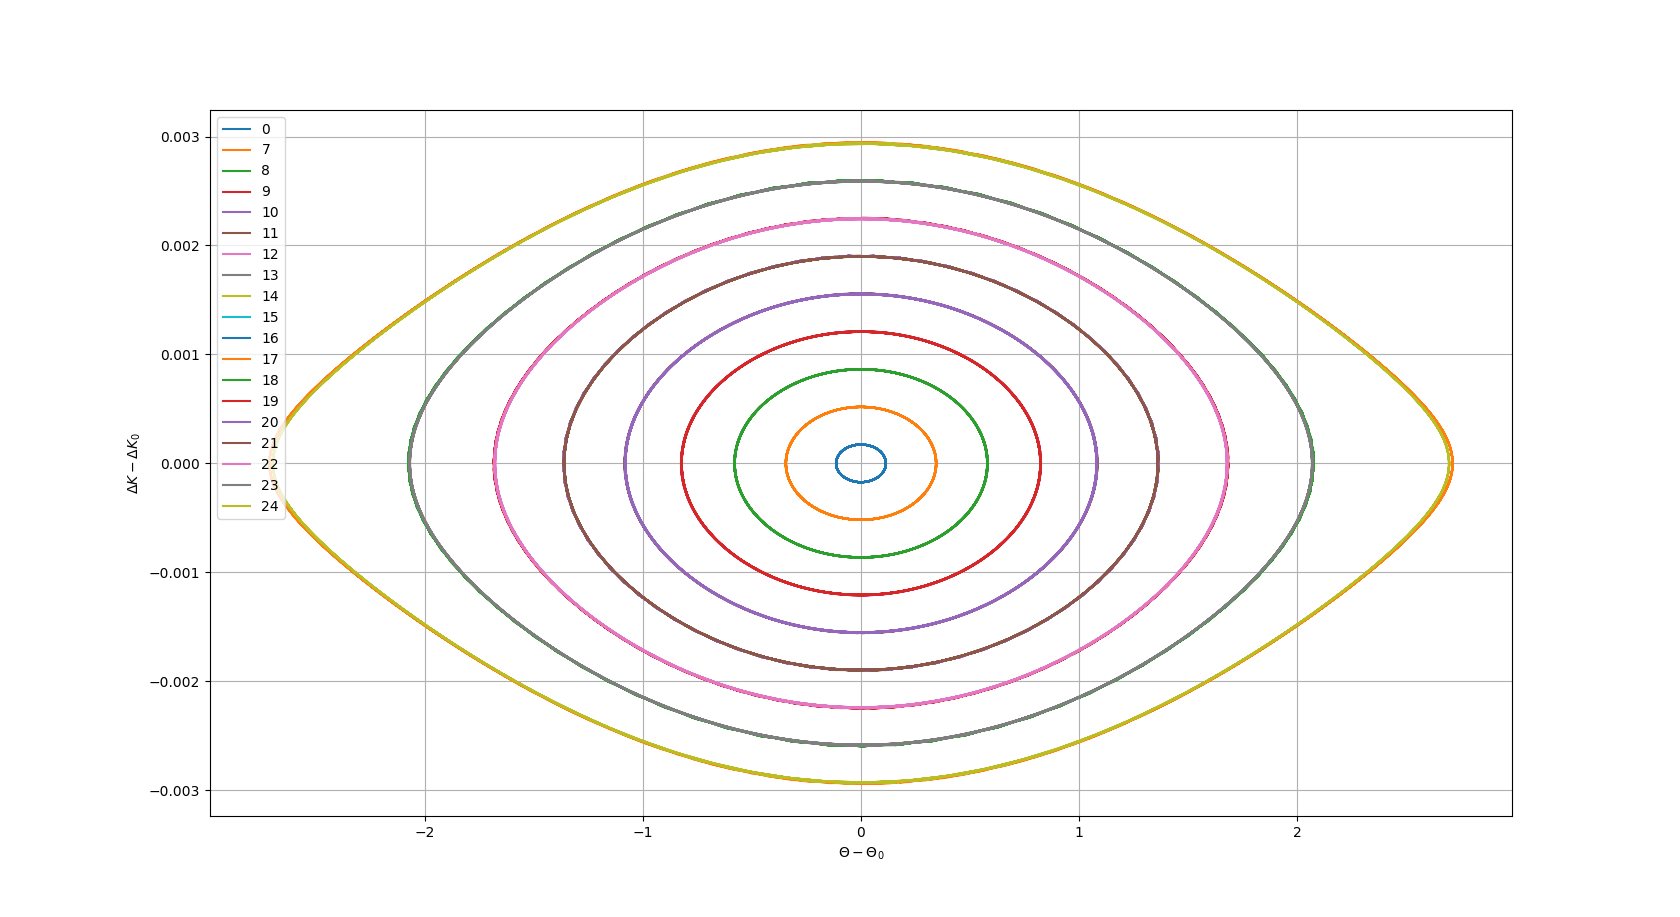
\includegraphics[scale=.25]{mean_dK_test_fishplot}
	\end{frame}
	\begin{frame}
		\centering
		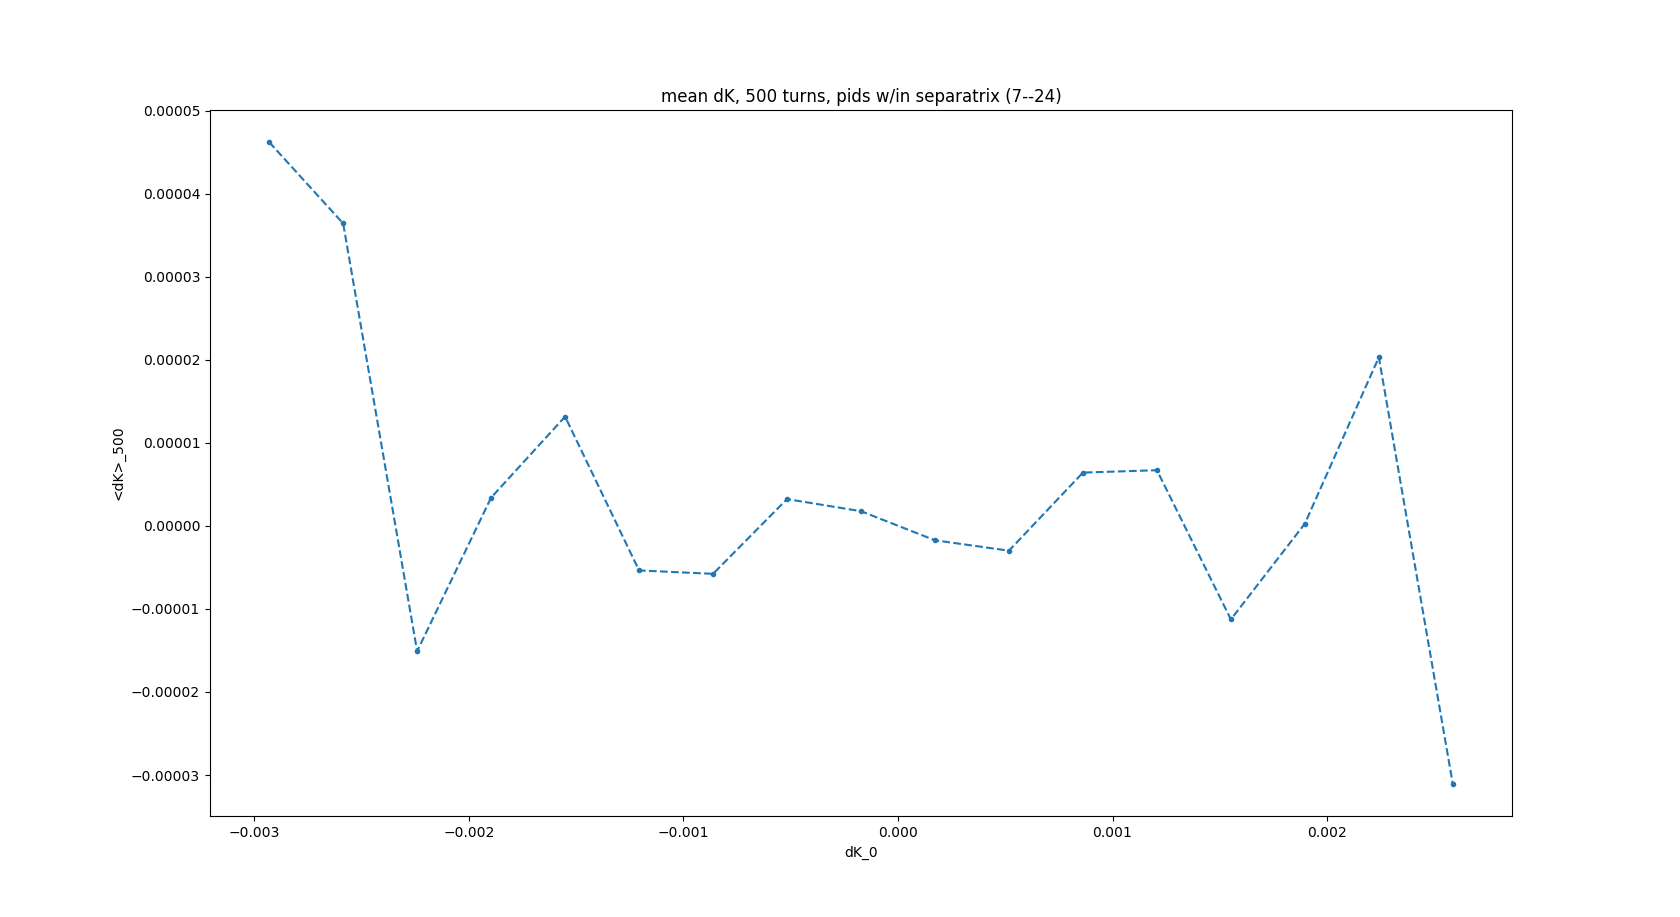
\includegraphics[scale=.3]{mean_dK_test_mean_dK_vs_dK0}
		\captionof{figure}{$\langle \Delta K\rangle$ vs $\Delta K_0$ after 500 turns (14 synchrotron oscillations)}
	\end{frame}
\begin{frame}
	\centering
	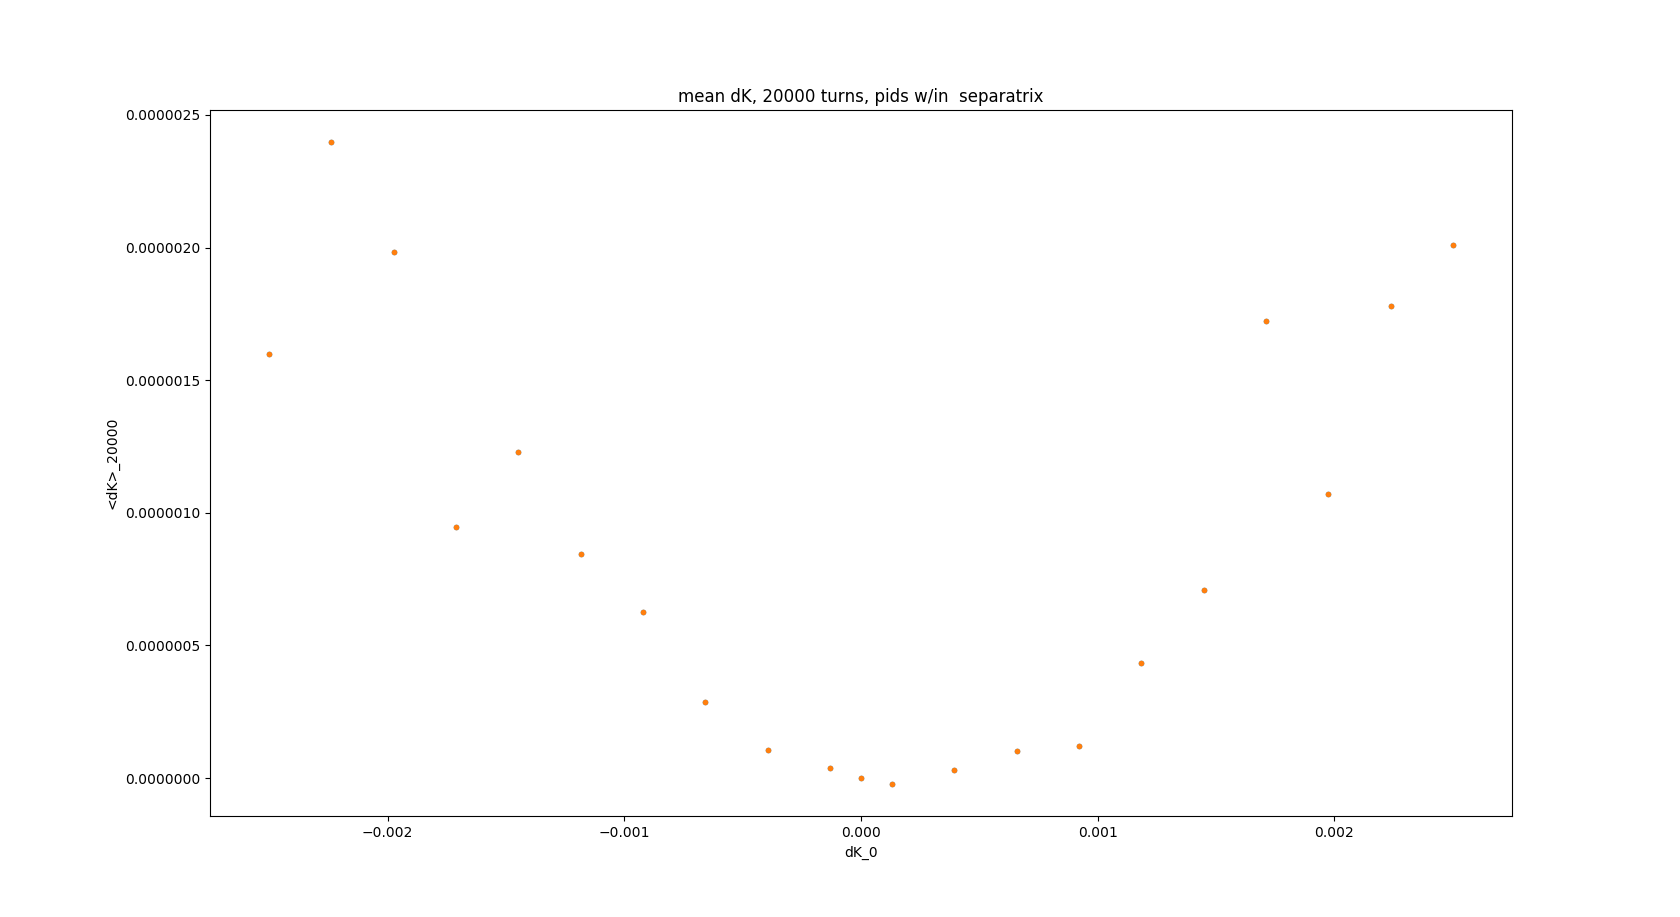
\includegraphics[scale=.3]{mean_dK_test_mean_dK_vs_dK0_20000trns_parabola}
	\captionof{figure}{$\langle \Delta K\rangle$ vs $\Delta K_0$ after 20,000 turns (571 synchrotron oscillations)}
\end{frame}
	
	\begin{frame}{Therefore...}
	\begin{itemize}
		\item Eremey Valetov compares a conventional Runge-Kutta 8-th order, step-size calibrated integrator (MSURK89) with COSY INFINITY with regard to run time;
		\item By my estimation, that integrator would take 32 hours to run a \textbf{single} simultation with just one realization of an imperfect 397-element FS lattice with the beam of 1000 particles for initial distribution;
		\item COSY INFINITY is an order of magnitude faster; that's manageable.
	\end{itemize}
	\end{frame}

\end{document}
